\documentclass{article}
\usepackage{graphicx}


\setlength{\parskip}{1em}

\begin{document}


\title{Resource Components}

Resource Components are ICE Components which contain a grid of visualization
resources. These resources can display files from a variety of sources,
such as CSV files or VisIt visualizations. Geometry and Mesh editors allow for
editing of shapes or meshes. Both can be added to an Item to offer visualization
of data.

\section{Prerequisites}

This tutorial assumes that the class you are writing already has an ICE Form. If
you are writing an extension of ICE's Item class, then the work of creating and
managing a Form is already done for you.

See the New Item Generation Tutorial, in the docs/newItemGeneration/ folder of 
the ICE repo for details on how to create an Item.

\section{Adding the Components}

First, add the neccesary imports for the components being added to your Item. 

\begin{verbatim}
import java.io.IOException;
import org.eclipse.core.resources.IFile;
import org.eclipse.core.resources.IProject;
import org.eclipse.core.runtime.IAdaptable;
import org.eclipse.eavp.viz.service.modeling.BasicView;
import org.eclipse.eavp.viz.service.modeling.ShapeController;
import org.eclipse.eavp.viz.service.modeling.ShapeMesh;
import org.eclipse.ice.datastructures.form.Form;
import org.eclipse.ice.datastructures.form.GeometryComponent;
import org.eclipse.ice.datastructures.form.MeshComponent;
import org.eclipse.ice.datastructures.form.ResourceComponent;
import org.eclipse.ice.datastructures.resource.VizResource;
\end{verbatim}

Next, copy and paste the following example code into your class.

\begin{verbatim}
//Create the resource component
ResourceComponent resourceComponent = new ResourceComponent();

//Set the component's data members
resourceComponent.setName("Resources");
resourceComponent.setDescription("Results");
resourceComponent.setId(2);

//Initialize the resources
VizResource csvResource = null;
VizResource visItResource = null;
IFile csvFile = null;
IFile visItFile = null;

//Open the files
csvFile = project.getFile("fib8.csv");
visItFile = project.getFile("wave.visit");

//If the file was found, create the CSV resource and add it to the component
try{
	if(csvFile.exists()){
		csvResource = new 
                    VizResource(csvFile.getLocation()
                    .toFile());
    	resourceComponent.addResource(csvResource);
	}
		        
	//If the file was found, create the VisIt resource and add it to 
	//the component
	if(visItFile.exists()){
		visItResource = new 
                    VizResource(visItFile.getLocation()
                    .toFile());
		resourceComponent.addResource(visItResource);
	}
}
catch(IOException e){
	e.printStackTrace();
}

//Create the geometry component
ShapeController geometryRoot = new ShapeController(new
    ShapeMesh(), new BasicView());
GeometryComponent geometryComponent = new 
    GeometryComponent();
geometryComponent.setGeometry(geometryRoot);

//Create mesh component
MeshComponent meshComponent = new MeshComponent();

//Add the components to the form
form.addComponent(resourceComponent);
form.addComponent(geometryComponent);
form.addComponent(meshComponent);	
\end{verbatim}

This code will add a Resource Component, Geometry Component, and Mesh Component
to your Item and load fib8.csv and wave.visit, which should be in the workspace
from your USB drive, into the Resource Component.


\section{Using the Resource Component}

\subsection{Establishing a VisIt Connection}

In order to visualize resources containing VisIt files, ICE must be connected to
a running VisIt installation. To set up this connection, select \texttt{Windows}
$\rightarrow$ \texttt{Preferences...} in ICE's menu bar. (On Mac OS X,
\texttt{Preferences} is instead located under \texttt{Eclipse} ICE in the menu
bar.)

\begin{center}
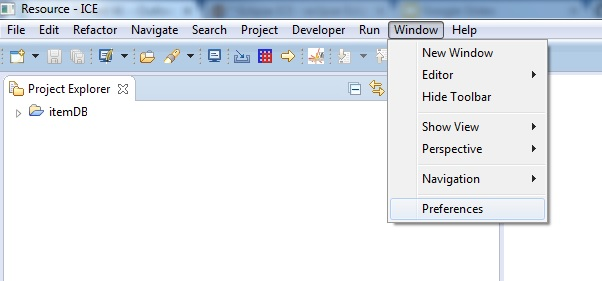
\includegraphics[width=12cm]{images/ICEPreferences}
\end{center}

Select \texttt{Visualization} $\rightarrow$ \texttt{VisIt} in the tree on the
left side of the \texttt{Preferences} window.

\begin{center}
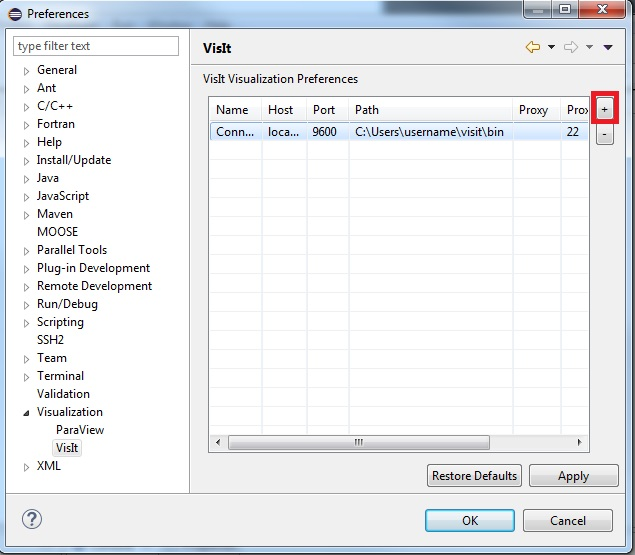
\includegraphics[width=12cm]{images/VisualizationPreferences}
\end{center}

Press the button with a "+" symbol in the upper right (highlighted in the image
above) to add a new row to the table. Click on the \texttt{Path} cell of the new
row and put the path of your installation of VisIt.

Press \texttt{Apply}, then \texttt{OK}, both in the lower right hand corner. ICE
will now open and connect to this VisIt installation each time ICE is opened.

\subsection{Managing the Resources}

Before opening your new Item, import your resources into the top level of your 
project. Afteword, you should notice a new tab inside containing your 
ResourceComponent. Its title will be whatever you set as its description when 
writing the code for it.

At the top left of the screen will be controls for the component's layout.

\begin{center}
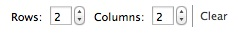
\includegraphics{images/ResourceComponentControls}
\end{center}

The \texttt{Clear} button will close all plots in the component. The other two
controls will allow you to specify the number of rows and columns in the grid.
Be careful when reducing them, as any plots which no longer fit in the grid will
be closed.

If you hover over a plot, a button will appear in the upper left hand corner.
Clicking it will close that plot. 

\begin{center}
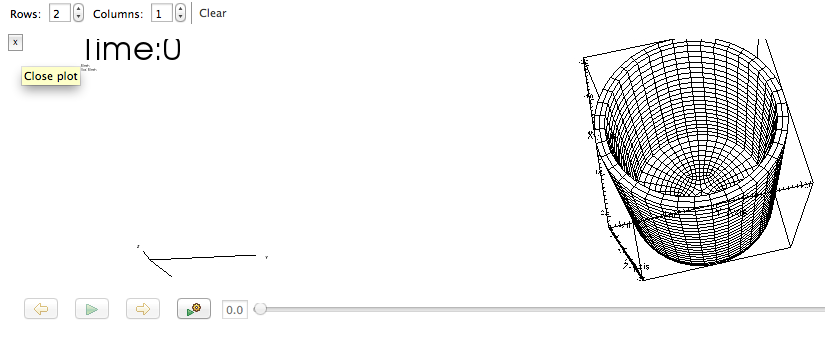
\includegraphics[width=12cm]{images/ClosePlotButton}
\end{center}

\subsection{Interacting with VisIt Plots}

\begin{center}
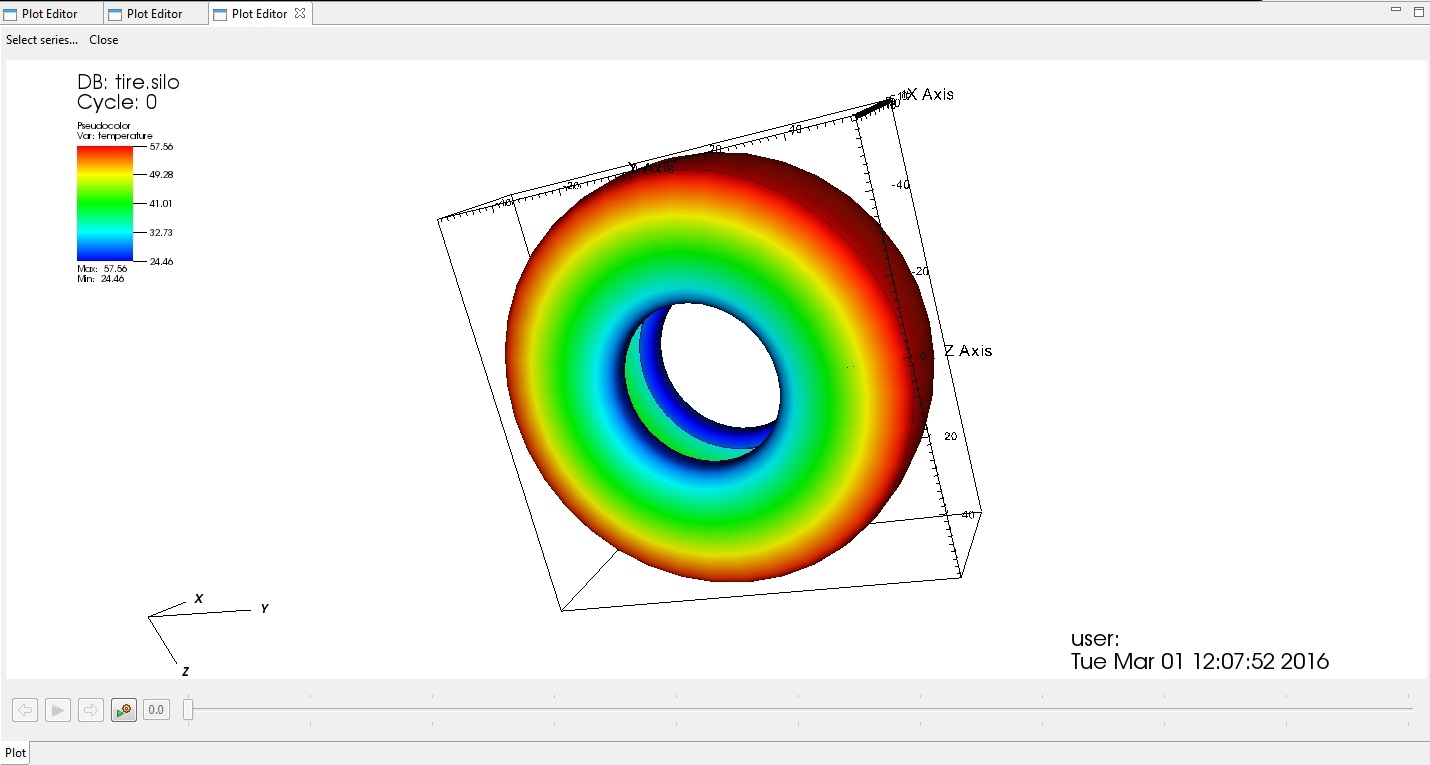
\includegraphics[width=12cm]{images/VisItPlot}
\end{center}

A VisIt plot will contain a 3D visualization of some model. You can click and
drag within the plot to rotate the image and zoom by scrolling your mouse wheel.
Right clicking in the plot will open a context menu, providing options for how
the model will be displayed.

At the bottom of the plot will be a series of controls for animation. If your
plot does not have time series data, they will be greyed out. 

\begin{center}

\includegraphics[width=12cm]{images/TimeSliderWidget} 
\end{center}

The plot can be set to display an arbitrary time step by either dragging the
slider or by typing a time into the box to its left.

\subsection{Interacting with CSV Plots}

\begin{center}
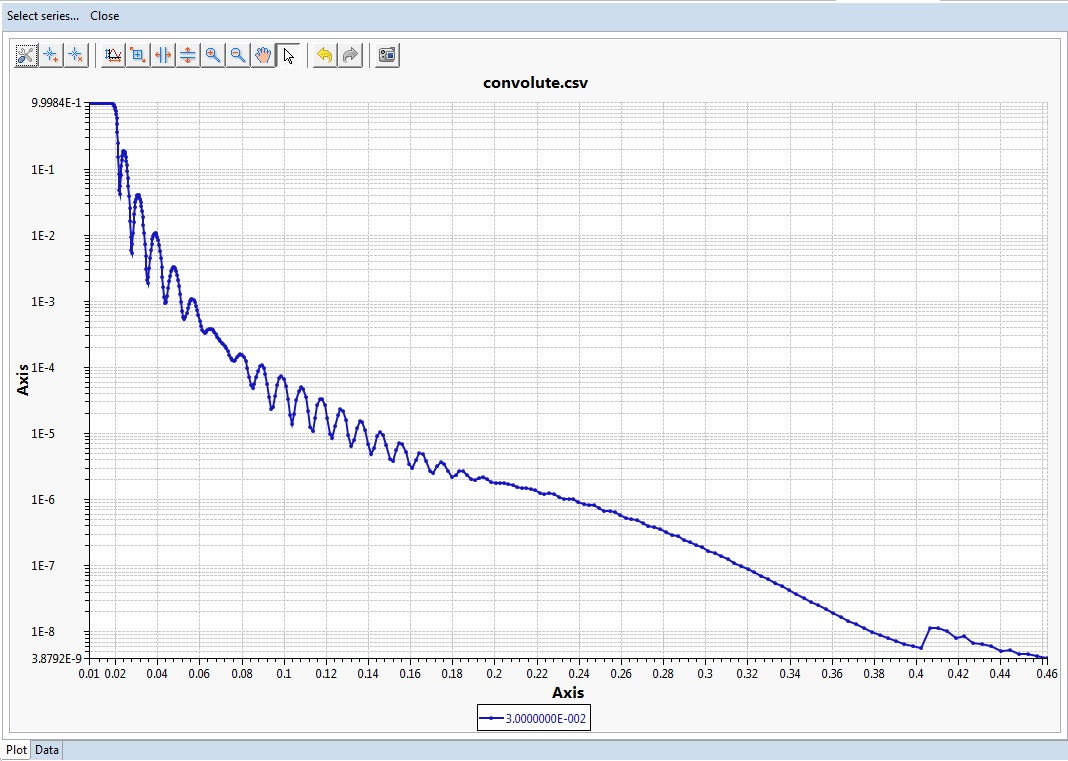
\includegraphics[width=12cm]{images/CSVGraph}
\end{center}

The top of the CSV plot has a row of buttons which control various aspects of
the graph's presentation. Right clicking will open a context menu allowing you
to choose which of the available series to plot.


\subsection{Editing 3D Structures}

ICE also contains capabilities to render graphics with the Geometry Editor and
Mesh Editor. Programatically populating these editors with custom input is
beyond the scope of this tutorial. However, what follows will be a brief
overview of the editors' functionality.

\subsubsection{The Geometry Editor}

The GeometryComponent you added to the form will create a new tab containing a
Geometry Editor. Shapes in the editor are structured as a Constructive Solid
Geometry Tree. 

Clicking the \texttt{Add Primitives} button will display a drop down of
primitive shapes which can be added to the scene.

\begin{center}
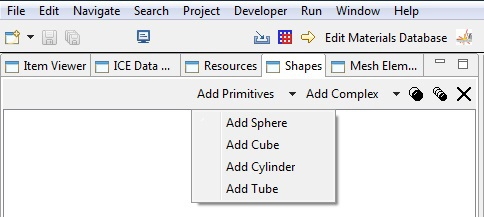
\includegraphics[width=12cm]{images/AddPrimitiveShape}
\end{center}

Complex shapes can similarly be added using the \texttt{Add Complex} button.

\begin{center}
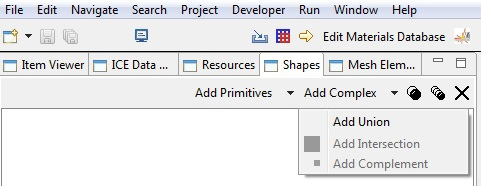
\includegraphics[width=12cm]{images/AddComplexShape}
\end{center}

Primitive shapes can be added under complex shapes by selecting anything beneath
the desired parent complex shape before adding the new primitive.

\begin{center}
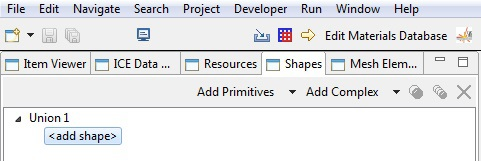
\includegraphics[width=12cm]{images/ComplexShapeTree}
\end{center}

The three other buttons are responsible for creating copies of or removing
selected shapes from the tree. 

The Transformation View, in the lower left, has spaces to set the rotation, scale, 
and translation of a selected object.

\begin{center}
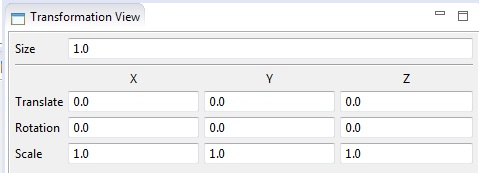
\includegraphics[width=12cm]{images/TransformationView}
\end{center}

\subsubsection{The Mesh Editor}

Like the Geometry Editor, the MeshComponent will create a Mesh Editor in your
form.

Clicking within the grid will create a vertex, until the fourth completes the
polygon.

\begin{center}
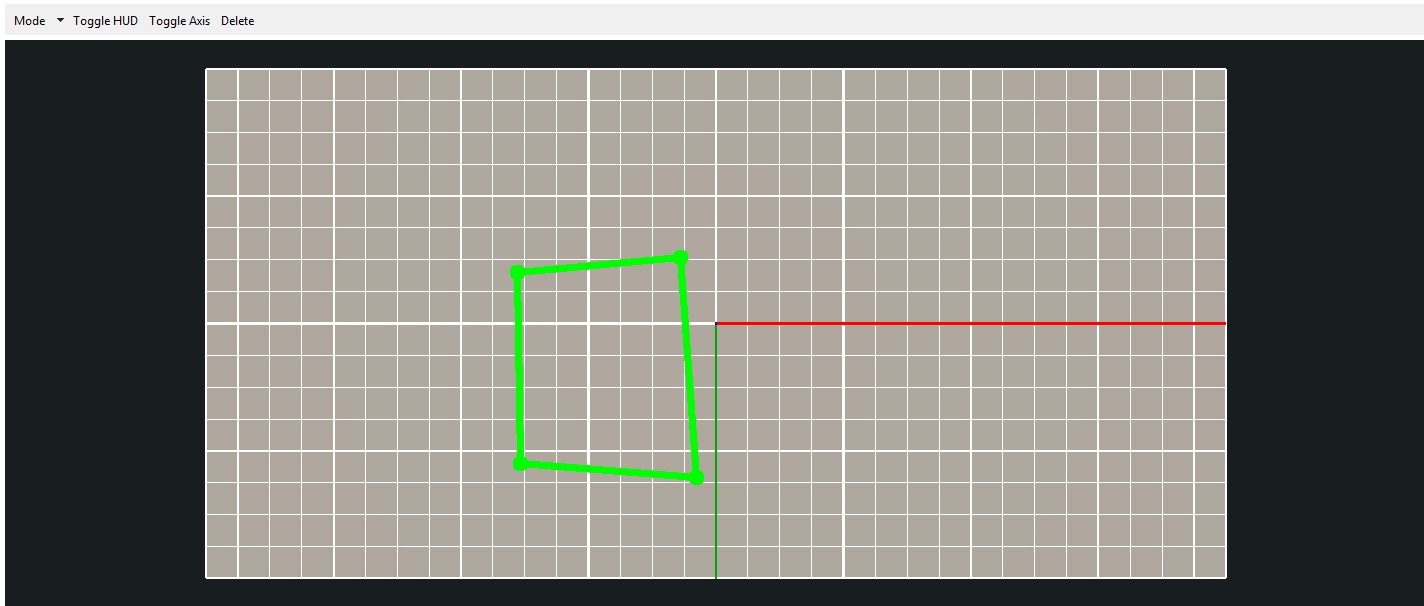
\includegraphics[width=12cm]{images/AddPolygon}
\end{center}

Click again to make the polygon permanent, signified by turning purple, or hit
\texttt{Esc} to cancel.

\begin{center}
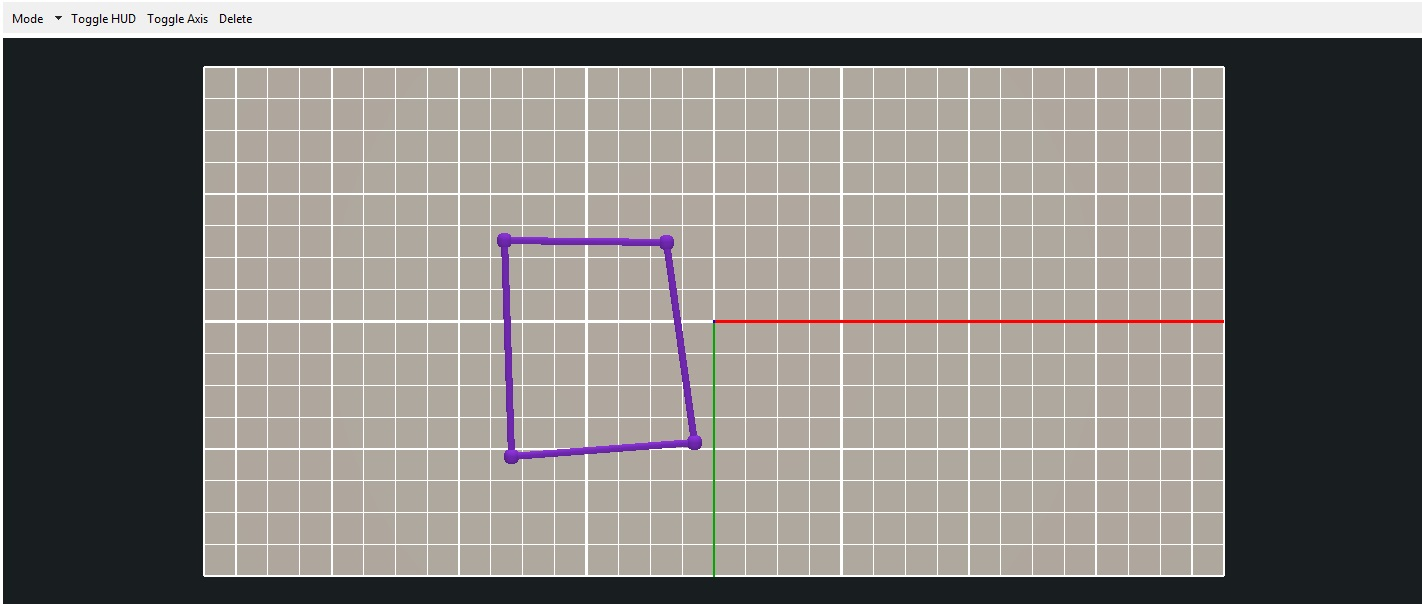
\includegraphics[width=12cm]{images/NewPolygon}
\end{center}

The \texttt{Mode} button in the top left allows you to switch between
\texttt{Add Elements} mode, used previously, and \texttt{Edit Elements} mode.

\begin{center}
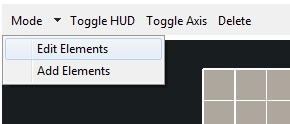
\includegraphics[width=12cm]{images/EditMode}
\end{center}

In edit mode, you can click a vertex (or vertices) to select them. 

\begin{center}
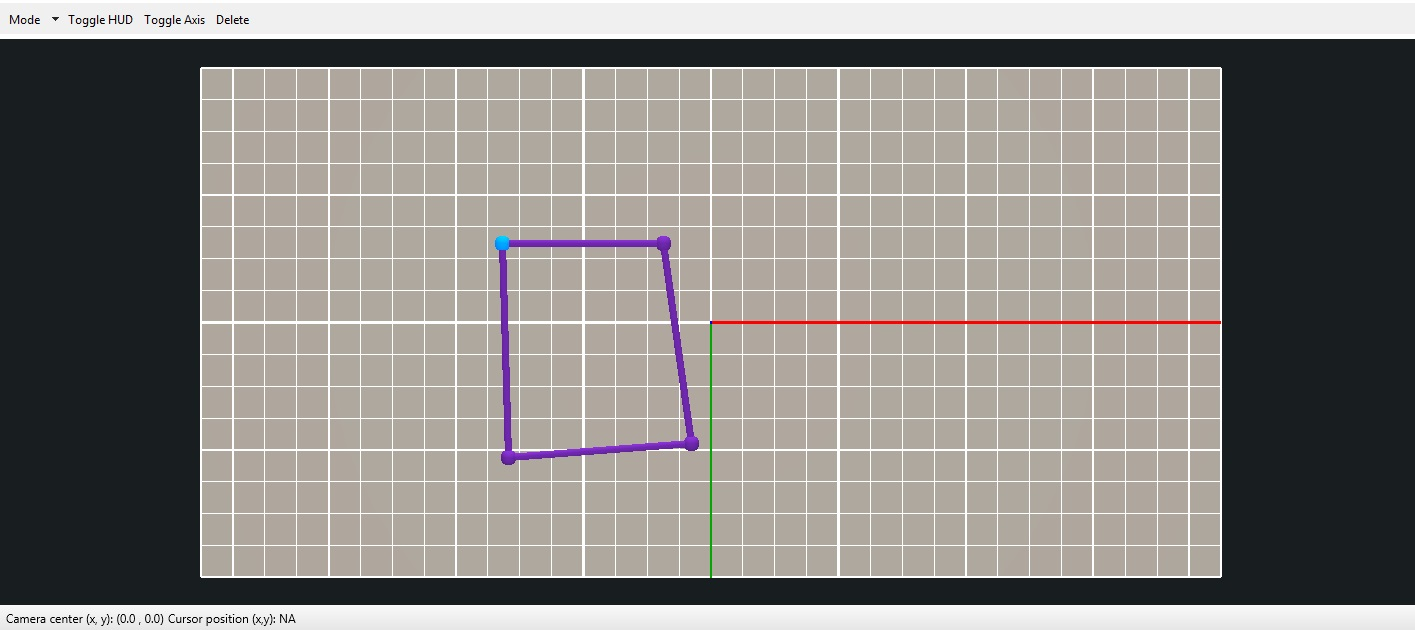
\includegraphics[width=12cm]{images/SelectedVertex}
\end{center}

You can click and drag a vertex to move all selected vertices around the grid.

\section{Further Reading}

This tutorial has only given a brief overview of the ways in which you can use
ICE's visualization tools. For more detailed information, look under the
\texttt{docs} folder in the ICE repository. The visualization folder contains a
tutorial on the CSV and VisIt plots, while the geometryEditor and meshEditor
folders have tutorials on the geometry and mesh editors, respectively. 

\end{document}
